\documentclass[a4paper]{ctexart}
\usepackage{xeCJK}
\usepackage{times}
\usepackage{setspace}
\usepackage{fancyhdr}
\usepackage{graphicx}
\usepackage{subfigure}
\usepackage{wrapfig}
\usepackage{array}
\usepackage{fontspec,xunicode,xltxtra}
\usepackage{titlesec}
\usepackage{titletoc}
\usepackage[titletoc]{appendix}
\usepackage[top=29mm,bottom=29mm,left=31.8mm,right=31.8mm]{geometry}
\usepackage{enumerate}
\usepackage{caption}
\usepackage{amsmath,bm}
\usepackage{cite}
\usepackage{algorithm}  
\usepackage{algorithmicx}  
\usepackage{algpseudocode}
\usepackage{lastpage}
\setmainfont{Times New Roman}
\setCJKmainfont[BoldFont={Songti SC Bold}]{SimSun}
\setCJKfamilyfont{heiti}{SimHei}
\renewcommand{\heiti}{\CJKfamily{heiti}\fontspec{Times New Roman}}

\newcommand{\mycaptionfont}{\heiti\zihao{5}}
\captionsetup[figure]{name={\mycaptionfont 图},labelsep=period}
\renewcommand{\captionfont}{\mycaptionfont}
\renewcommand{\captionlabelfont}{\mycaptionfont}

\ctexset {
	section = {
		number = \chinese{section},
		format = \zihao{4}\bfseries,
	},
	subsection = {
		number = \arabic{section}.\arabic{subsection},
		format = \zihao{-4}\bfseries,
	}
}


\fancypagestyle{plain}{\pagestyle{fancy}}%改变章节首页页眉
\pagestyle{fancy}
\lhead{传感器网络连通性实验}
\chead{传感器网络实验报告}
\rhead{1030616134~尹达恒}
\cfoot{\thepage\quad/\quad\pageref{LastPage}}

\begin{document}
\begin{spacing}{1}
\zihao{-4}
\section{实验名称:传感器网络连通性实验}
\begin{tabular}{lll}
	班级:物联网1601&姓名:尹达恒&学号:1030616134\\
\end{tabular}
\section{实验要求}
\begin{enumerate}[1、]
	\item 编写一个能够按照指定的传感器数量和传感器布置范围随机生成传感器网络邻接矩阵的算法;
	\item 编写一个能够根据传感器网络邻接矩阵和传感器通信半径计算网络连通度的算法;
	\item 在不同传感器数量条件下,固定随机生成传感器的数量,绘制多条传感器通信半径-传感器网络连通度曲线;
	\item 在不同通信半径条件下,固定传感器通信半径,绘制多条传感器数量-传感器网络连通度曲线。
\end{enumerate}

\section{实验步骤}
\subsection{邻接矩阵随机生成算法}
为简便起见,假定传感器布置在一个方形区域内,传感器网络整体为一个无向图,传感器邻接矩阵表示传感器之间的物理间距。指定传感器数量$n$和布置范围边长$d$随机生成传感器网络邻接矩阵$G$的算法可以简化为:
\begin{enumerate}
	\item 随机生成$n$个传感器的位置$P=\{(x_i,y_i)|0<x_i<d,0<y_i<d,0<i\le n\}$;
	\item 计算各个传感器之间的距离,形成邻接矩阵$G$。
\end{enumerate}
算法如下:
\begin{algorithm}
	\caption{邻接矩阵生成算法}
	\label{a11}
	\begin{algorithmic}[1]
		\Require 传感器数量$n$、传感器布置范围边长$d$
		\Ensure $n$为自然数、$d>0$
		\Function {AdjacencyMatrix}{$n$,$d$}
		\State $P\gets n$位随机数组$\{(x_i,y_i)|0<x_i<d,0<y_i<d,0<i\le n\}$
		\State $G\gets \{G_{ij}\}=\sqrt{(x_i-x_j)^2+(y_i-y_j)^2}$
		\State \Return{$G$}  
		\EndFunction  
	\end{algorithmic}
\end{algorithm}
在实际程序中,$\{G_{ij}\}$的计算使用Pytorch中的矩阵操作,调用GPU进行并行计算以提升速度。

\subsection{网络连通度计算方法}
已知邻接矩阵$G$和传感器通信半径$r$求网络连通度的算法可以分为两步:首先由阵$G$和离$r$求出传感器网络的连通性矩阵$C$,然后由$C$次方求和求得网络的总连通度。

连通性矩阵$C$的求得是对网络$G$中节点连通性进行依次判断的过程,对邻接矩阵$G$中的每个元素$G_{ij}$,如果$G_{ij}<r$,则$C_{ij}=1$表示节点间连通,否则$C_{ij}=0$表示节点间不连通。

按照网络连通度的有关定理,给定网络连通性矩阵$C$求网络连通度的方法可以用一系列矩阵次方求和实现。对于一个给定的无向图连通性矩阵$C$,网络的第$k$跳连通性可以用$C$的$k$次方表示:$C^k$。$C^k$中元素为0表示节点$k$跳不连通,元素不为0表示节点$k$跳连通。一个有$n$个节点的网络的总连通性矩阵$S$可以通过各跳的连通性矩阵求和来计算:$S=\sum_{k=1}^n C^k$。网络连通性可以用总连通性矩阵$S$中是否有0元素表示:如果总连通性矩阵$S$中没有0元素说明网络连通,反之说明网络不连通。为提升计算速度,当计算到某一跳的总连通性矩阵元素全部为1时可以直接得到矩阵100\%连通而立即停止计算。故可得如Algorithm\ref{a12}的连通度计算方法。
\begin{algorithm}
	\caption{网络连通度计算方法}
	\label{a12}
	\begin{algorithmic}[1]
		\Require 邻接矩阵$G$、传感器数量$n$、传感器通信半径$r$
		\Ensure $n$为自然数、$G$为$n\times n$对称矩阵对角线元素为0、$r\ge 0$
		\Function {CalculateConnectivity}{$G$,$n$,$r$}
		\State $C\gets \{C_{ij}\}=\{
		\begin{array}{r}
		1\quad G_{ij}<r\\
		0\quad G_{ij}\ge r\\
		\end{array}$
		\State $C'\gets C$
		\State $S\gets C$
		\For{$k = 1 \to n$}
		\If{$S$中没有0元素}
		\State \Return{$1$}
		\EndIf
		\State $C'\gets C'\times C$
		\State $S\gets S+C'$
		\EndFor
		\If{$S$中没有0元素}
		\State \Return{$1$}
		\EndIf
		\State \Return{$0$}
		\EndFunction
	\end{algorithmic}
\end{algorithm}
在实际程序中,$\{C_{ij}\}$、$C'\gets C'\times C$和$S\gets S+C'$的计算使用Pytorch中的矩阵操作,调用GPU进行并行计算以提升速度。

\subsection{绘制传感器通信半径-传感器网络连通度曲线}
绘制传感器通信半径-传感器网络连通度曲线时,传感器的数量$n$和布置范围边长$d$固定,传感器通信半径从0开始增加到$d$,可获得一系列传感器通信半径-传感器网络连通度对应关系,以通信半径为$x$轴,网络连通度为$y$轴,绘制出的曲线即为一条传感器通信半径-传感器网络连通度曲线。改变传感器的数量$n$多次绘制,可以得到不同传感器的数量下传感器通信半径-传感器网络连通度曲线。为减小偶然性,每次求传感器网络连通度时都要多次计算取平均值。算法如Algorithm\ref{a21}。
\begin{algorithm}
	\caption{绘制传感器通信半径-传感器网络连通度曲线}
	\label{a21}
	\begin{algorithmic}[1]
		\Require 传感器布置范围边长$d$,重复计算次数$a$,传感器数量限制$n_{max}$
		\For{$n=2 \to n_{max}$}
		\State$x\gets$空数组
		\State$y\gets$空数组
		\For{$r=0 \to \sqrt{2}d$}
		\State$average=0$
		\For{$a$次循环}
		\State$G=$\Call{AdjacencyMatrix}{$n$,$d$}
		\State$t=$\Call{CalculateConnectivity}{$G$,$n$,$r$}
		\State$average=average+t$
		\EndFor
		\State$average=average/a$
		\State$r$值放入数组$x$
		\State$average$值放入数组$y$
		\EndFor
		\State 绘制一条$x,y$关系曲线
		\EndFor
	\end{algorithmic}
\end{algorithm}

\subsection{绘制传感器数量-传感器网络连通度曲线}
绘制传感器数量-传感器网络连通度曲线时,传感器的通信半径$r$和布置范围边长$d$固定,传感器数量从2开始依次增加,可获得一系列传感器数量-传感器网络连通度对应关系,以传感器数量为$x$轴,网络连通度为$y$轴,绘制出的曲线即为一条传感器数量-传感器网络连通度曲线。改变传感器的通信半径$r$多次绘制,可以得到不同通信半径下传感器数量-传感器网络连通度曲线。为减小偶然性,每次求传感器网络连通度时都要多次计算取平均值。算法如Algorithm\ref{a22}。

\begin{algorithm}
	\caption{绘制传感器通信半径-传感器网络连通度曲线}
	\label{a22}
	\begin{algorithmic}[1]
		\Require 传感器布置范围边长$d$,重复计算次数$a$,传感器数量限制$n_{max}$
		\For{$r=0 \to \sqrt{2}d$}
		\State$x\gets$空数组
		\State$y\gets$空数组
		\For{$n=2 \to n_{max}$}
		\State$average=0$
		\For{$a$次循环}
		\State$G=$\Call{AdjacencyMatrix}{$n$,$d$}
		\State$t=$\Call{CalculateConnectivity}{$G$,$n$,$r$}
		\State$average=average+t$
		\EndFor
		\State$average=average/a$
		\State$n$值放入数组$x$
		\State$average$值放入数组$y$
		\EndFor
		\State 绘制一条$x,y$关系曲线
		\EndFor
	\end{algorithmic}
\end{algorithm}

\section{实验结果}
\subsection{传感器通信半径-传感器网络连通度曲线}
传感器布置范围边长$d=10$、重复计算次数$a=2000$时,取$n\in\{10,20,30,40,50\}$,$r$为0.01$\sim$10之间间隔0.1的100个浮点数,绘制传感器通信半径-传感器网络连通度曲线,程序运行环境为Windows 10 + CUDA 10.0 + Python 3.6 + Pytorch 1.0,CPU为Intel i5-7200U,GPU为Nvidia GeForce 940MX,程序运行时间约865.8s,计算结果如图\ref{f1}。

\subsection{传感器数量-传感器网络连通度曲线}
传感器布置范围边长$d=10$、重复计算次数$a=2000$时,取$r\in\{2,4,6,8,10\}$,$n$为1$\sim$25共25个整数,绘制传感器数量-传感器网络连通度曲线,程序运行环境和硬件配置同上,程序运行时间约71.86s,计算结果如图\ref{f2}。

\begin{figure}[htbp]
	\begin{minipage}[t]{0.5\textwidth}
		\centering
		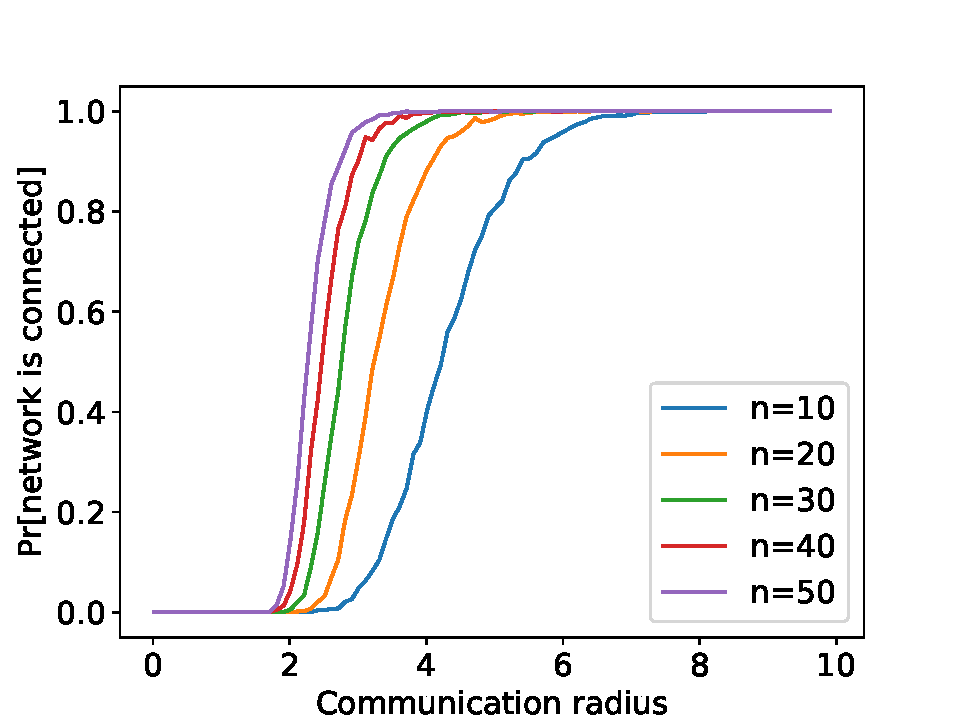
\includegraphics[width=1.1\textwidth, keepaspectratio]{figure/Figure_1.pdf}\\
		\caption{通信半径-网络连通度曲线}\label{f1}
	\end{minipage}%
	\hfill
	\begin{minipage}[t]{0.5\textwidth}
		\centering
		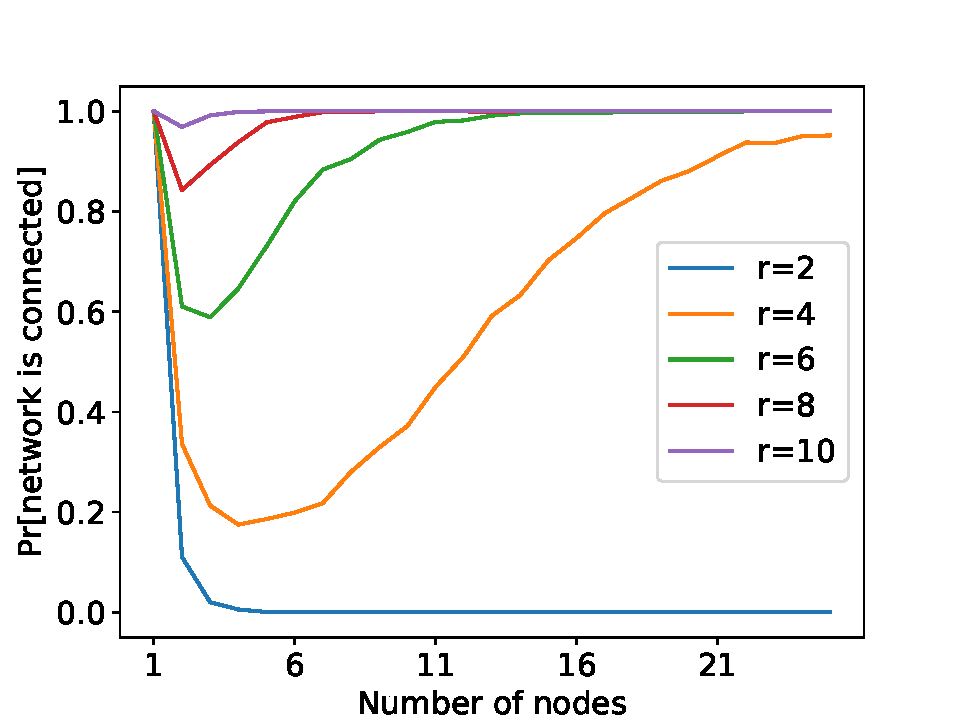
\includegraphics[width=1.1\textwidth, keepaspectratio]{figure/Figure_2.pdf}\\
		\caption{传感器数量-网络连通度曲线}\label{f2}
	\end{minipage}
\end{figure}

\section{实验结果分析}
由图\ref{f1}可知,在传感器数目一定的情况下,传感器的通信半径越大,网络的连通度越高;图\ref{f2}可知,在传感器通信半径一定的情况下,单位面积内的传感器的数目越多,网络的连通度越高。但是不管是增加传感器数目还是提高传感器的通信半径,网络的连通度的增加都是有极限的,传感器的通信半径或传感器数目提高到一定程度都会造成网络资源的浪费,在实际传感网系统设计过程中应有所取舍。
\end{spacing}
\end{document}